% =============================================================
%  System Design Document – Emergency Stop System
%  Kurs: Software Engineering (DHBW Ravensburg, Campus Friedrichshafen)
%  Gruppe: Die Drei Muskeltiere
%  Stand: März 2026
% =============================================================
\documentclass[12pt, a4paper]{article}

% --- Sprache & Kodierung ---
\usepackage[T1]{fontenc}
\usepackage[utf8]{inputenc}
\usepackage[ngerman]{babel}

% --- Typografie & Layout ---
\usepackage[
  top=2.5cm, bottom=2.5cm,
  left=3cm,  right=2.5cm
]{geometry}
\usepackage{microtype}
\usepackage{parskip}
\usepackage{lmodern}

% --- Grafiken ---
\usepackage{graphicx}
\usepackage{float}
% Suchpfad für Diagramme (relativ zu diesem Dokument)
\graphicspath{{../Diagram_SE/}}

% --- Farben & Highlighting ---
\usepackage{xcolor}
\definecolor{todocolor}{RGB}{200,0,0}
\definecolor{assumpcolor}{RGB}{0,100,180}
\definecolor{tableheader}{RGB}{230,230,230}

% --- Mathematik ---
\usepackage{amsmath}
\usepackage{amssymb}

% --- Tabellen ---
\usepackage{booktabs}
\usepackage{array}
\usepackage{longtable}

% --- Kopf-/Fußzeilen ---
\usepackage{fancyhdr}
\setlength{\headheight}{14pt}
\pagestyle{fancy}
\fancyhf{}
\fancyhead[L]{\small System Design Document – Emergency Stop}
\fancyhead[R]{\small Die Drei Muskeltiere}
\fancyfoot[C]{\thepage}
\renewcommand{\headrulewidth}{0.4pt}

% --- Hyperlinks & PDF-Metadaten ---
\usepackage[
  colorlinks=true,
  linkcolor=black,
  urlcolor=blue,
  citecolor=black,
  pdftitle={System Design Document – Emergency Stop},
  pdfauthor={Die Drei Muskeltiere},
  pdfsubject={Software Engineering DHBW},
  bookmarks=true
]{hyperref}

% --- Hilfs-Kommandos ---
% Sichtbare TODO-Markierung im PDF
\newcommand{\todo}[1]{%
  \textcolor{todocolor}{\textbf{[TODO: #1]}}%
}
% Sichtbare Annahmen-Markierung
\newcommand{\assumption}[1]{%
  \textcolor{assumpcolor}{\textit{[Annahme: #1]}}%
}
% Abschnittsweiser Platzhalter
\newcommand{\todobox}[1]{%
  \vspace{0.5em}%
  \noindent\colorbox{yellow!30}{%
    \parbox{\dimexpr\linewidth-2\fboxsep\relax}{%
      \textcolor{todocolor}{\textbf{TODO:} #1}%
    }%
  }%
  \vspace{0.5em}%
}

% =============================================================
\begin{document}

% --- Titelseite ---
\begin{titlepage}
  \centering
  \vspace*{2cm}
  {\LARGE\bfseries System Design Document\par}
  \vspace{0.5cm}
  {\Large Emergency Stop System\par}
  \vspace{0.5cm}
  {\large Autonome Fahrzeugplattform – Truck\par}
  \vspace{2cm}
  \rule{\linewidth}{0.4pt}\\[0.5cm]
  {\large
    \textbf{Kurs:} Software Engineering\\[0.3cm]
    \textbf{Gruppe:} Die Drei Muskeltiere\\[0.3cm]
    \textbf{DHBW Ravensburg, Campus Friedrichshafen}\\[0.3cm]
    \textbf{Datum:} März 2026\\[0.3cm]
  }
  \rule{\linewidth}{0.4pt}
  \vfill
  \begin{tabular}{ll}
    \textbf{Bewertungsgewichtung:} & 75\,\% Architektur-Dokumentation\\
                                   & 25\,\% Detailed Design\\
  \end{tabular}
\end{titlepage}

% --- Inhaltsverzeichnis ---
\tableofcontents
\clearpage

% --- Abbildungsverzeichnis ---
\listoffigures
\clearpage

% --- Kapitel ---
% =============================================================
%  Kapitel 1 – Einleitung
% =============================================================
\section{Einleitung}
\label{sec:einleitung}

Dieses Dokument beschreibt das \textbf{Program Design} des verteilten Not-Halt-Systems
einer autonomen Fahrzeugplattform (Truck).
Es hat den Charakter eines \ac{SDD} und dokumentiert
die Softwarearchitektur sowie das detaillierte Design des Teilsystems \textbf{Emergency Stop}.

\subsection{Scope}
\label{sec:scope}

\begin{itemize}
  \item \textbf{In Scope:} Software im Truck (Jetson Nano, Arduino Mega Master,
        Arduino Mega Slave), Architektur, Kommunikationsschnittstellen,
        Emergency-Stop-Logik, Boundary Conditions.
  \item \textbf{Out of Scope:} PC-Anwendung, \ac{ROS}-Integration, \ac{WLAN}-Kommunikation,
        Details der Sensor-Fusion (wird als Blackbox behandelt).
  \item \textbf{Vereinfachungen:}
        LiDAR liefert direkt die Distanz zum nächstliegenden Objekt;
        Sensor-Fusion ist vorgelagert und für dieses Dokument transparent.
\end{itemize}

\subsection{Ziel des Dokuments}
\label{sec:ziel}

Das \ac{SDD} richtet sich an Entwicklerinnen und Entwickler, die
\begin{enumerate}
  \item die Gesamtarchitektur und die Subsystem-Verantwortlichkeiten verstehen,
  \item das Deployment auf den Hardwareeinheiten nachvollziehen,
  \item das dynamische Verhalten (Sequenzen, Boundary Conditions) analysieren und
  \item das Emergency-Stop-Modul detailliert implementieren wollen.
\end{enumerate}

\newpage
\subsection{Abgrenzung Normal Operation vs.\ Emergency Stop}
\label{sec:abgrenzung}

Das System unterscheidet zwei Betriebsmodi (vgl.\ Abbildung~\ref{fig:zone_definition}):


\begin{description}
  \item[Normal Operation (Gelb/Grün)]
    Der \emph{\ac{TTC}-Observer} überwacht die Umgebung und erlaubt
    eine automatische Reaktion auf Hindernisse.  Der Fahrvorgang wird angepasst,
    das Fahrzeug kann aber weiterfahren.  \ac{TTC} ist \textbf{kein} Bestandteil des
    Emergency-Stop-Moduls.
  \item[Safety Zone / Emergency Stop (Rot)]
    Sobald ein Objekt die rote Sicherheitszone unterschreitet, ein Pilzknopf gedrückt
    oder ein Fronttaster ausgelöst wird, übernimmt der \emph{Emergency Stop}.
    Das Fahrzeug bleibt stehen, bis eine \textbf{manuelle Freigabe} erfolgt
    (Guard-Bedingung: Safety-Zone nicht mehr aktiv, kein Fehler).
\end{description}


\begin{figure}[H]
  \centering
  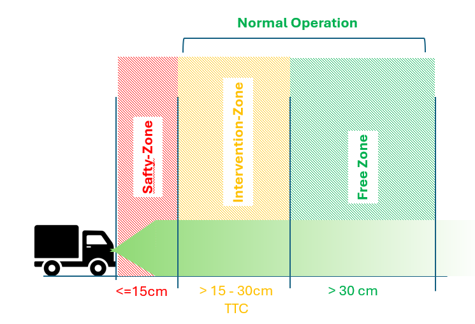
\includegraphics[width=0.95\textwidth]{Zone_Definition.png}
  \caption{Zone Definition (Ref. Aufgabenstellung \cite{PPT_SE_Operation_Zones})}
  \label{fig:zone_definition}
\end{figure}


% =============================================================
%  Kapitel 2 – Gesamtarchitektur
% =============================================================
\section{Gesamtarchitektur des Systems}
\label{sec:gesamtarchitektur}

\subsection{Systemkontext}
\label{sec:systemkontext}

Das Fahrzeug besteht aus drei physisch getrennten Recheneinheiten,
die über definierte Kommunikationskanäle miteinander verbunden sind:

\begin{itemize}
  \item \textbf{Jetson Nano} – Hochleistungs-Recheneinheit für Wahrnehmung und autonome Logik.
  \item \textbf{Arduino Mega Master} – Kommunikations-Gateway zwischen Jetson und Slave.
  \item \textbf{Arduino Mega Slave} – Sicherheitskritische Einheit nahe der Motorsteuerung;
        hier läuft der Emergency Stop.
\end{itemize}

Die Kommunikation erfolgt über:
\begin{itemize}
  \item \textbf{LAN} (Jetson Nano $\leftrightarrow$ Arduino Mega Master)
  \item \textbf{CAN-Bus} (Arduino Mega Master $\leftrightarrow$ Arduino Mega Slave)
\end{itemize}

Die Platzierung des Emergency Stop auf dem Slave minimiert Kommunikationsverzögerungen
zur Motorsteuerung (\emph{DriveControlUnit}) und stellt eine deterministische
Reaktionszeit sicher.

\begin{figure}[H]
  \centering
  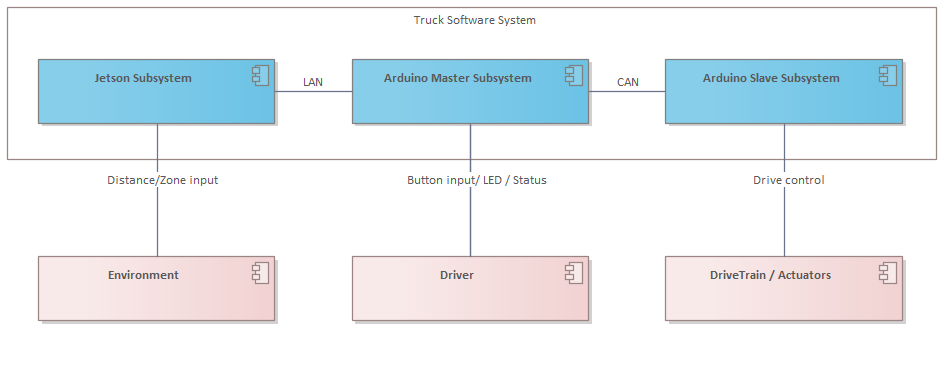
\includegraphics[width=0.95\textwidth]{01_Context}
  \caption{Kontextdiagramm – Systemgrenzen und externe Akteure}
  \label{fig:context}
\end{figure}

\subsection{Logische Systemstruktur (Component Overview)}
\label{sec:component_overview}

Die logische Architektur zeigt die funktionale Zerlegung des Systems in Subsysteme.
Abbildung~\ref{fig:component_overview} gibt einen Überblick.

\begin{figure}[H]
  \centering
  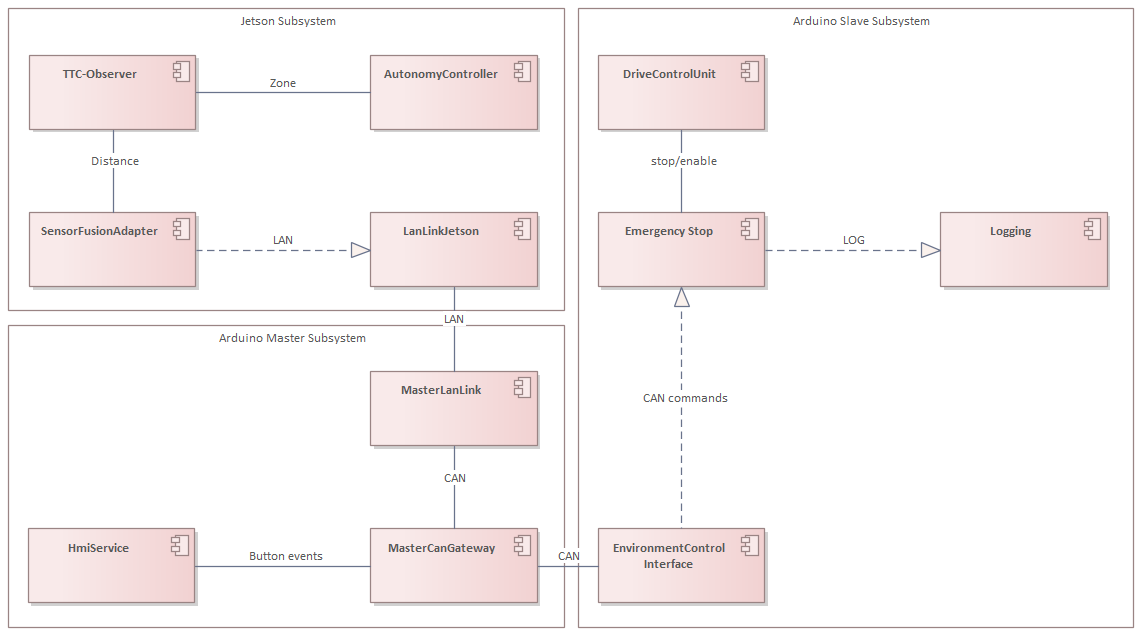
\includegraphics[width=0.95\textwidth]{02_Component_Overview}
  \caption{Komponentenübersicht – logische Systemstruktur}
  \label{fig:component_overview}
\end{figure}

Wesentliche Eigenschaften der Architektur:
\begin{itemize}
  \item Der \textbf{TTC-Observer} verarbeitet Sensordaten zur Bestimmung der Fahrzone
        (Grün/Gelb) und gehört ausschließlich zur \emph{Normal Operation}.
  \item Der \textbf{Emergency Stop} verarbeitet ausschließlich CAN-basierte Kommandos
        und ist von der Autonomie-Logik entkoppelt.
  \item Sensorik wird über das \texttt{EnvironmentControl}-Interface in CAN-Nachrichten
        übersetzt (Sensor-Fusion als Blackbox).
  \item Das \textbf{Logging}-Modul ist als separates Querschnittsmodul modelliert;
        es wird von Emergency Stop bei jeder Zustandsänderung aufgerufen.
  \item Eine direkte Abhängigkeit zwischen TTC-Observer und Emergency Stop
        \textbf{existiert nicht} – dies sichert die Unabhängigkeit der Sicherheitsfunktion.
\end{itemize}

\subsection{Subsystem-Verantwortlichkeiten und Klassendiagramme}
\label{sec:klassendiagramme}

Die folgenden Klassendiagramme zeigen Attribute und öffentliche Operationen
pro Hardware-Subsystem.

\subsubsection{Jetson Nano – Klassen}

\begin{figure}[H]
  \centering
  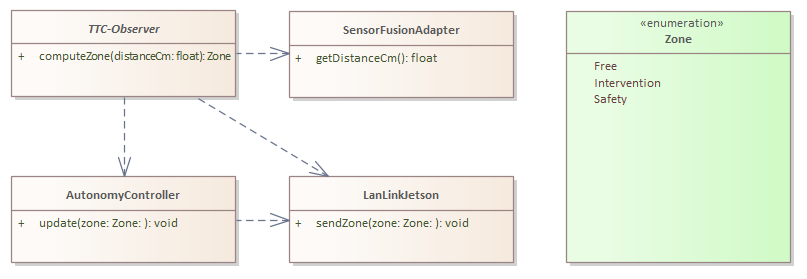
\includegraphics[width=0.95\textwidth]{02_Jetson_ClassDiagram}
  \caption{Klassendiagramm Jetson Nano: Autonomie-/Wahrnehmungs-Subsystem}
  \label{fig:jetson_classes}
\end{figure}

Hauptverantwortlichkeiten des Jetson-Subsystems:
\begin{description}
  \item[\texttt{AutonomyController}]
    Koordiniert autonomes Fahrverhalten; empfängt Zonenstatus vom TTC-Observer.
  \item[\texttt{TTCObserver}]
    Berechnet Time-To-Collision aus Sensordaten; sendet ZoneUpdate-Kommandos
    (Normal/Warnung). Zuständig für Gelb- und Grün-Zonen.
  \item[\texttt{SensorFusionAdapter}]
    Abstrahiert die Sensor-Fusion (Kamera + LiDAR); liefert normierte
    Distanz-/Objektdaten. Intern als Blackbox behandelt.
\end{description}

\subsubsection{Arduino Mega Master – Klassen}

\begin{figure}[H]
  \centering
  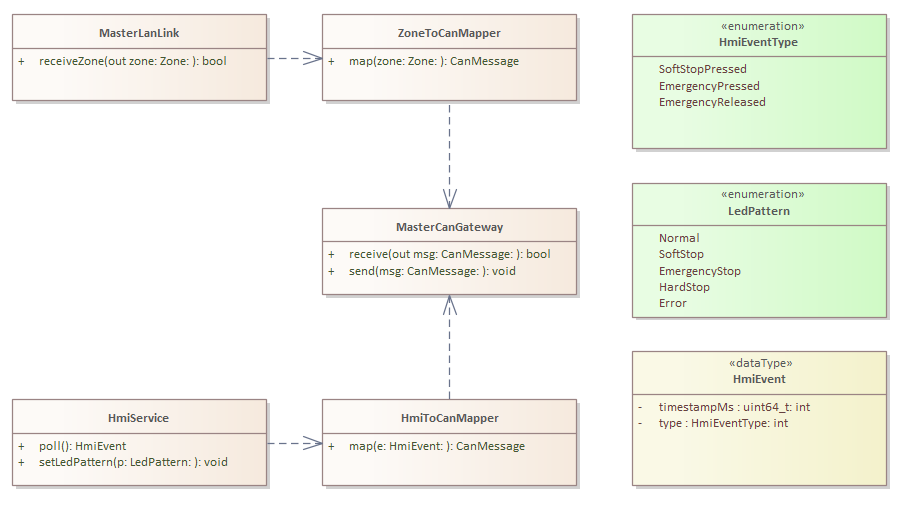
\includegraphics[width=0.95\textwidth]{02_Master_ClassDiagram}
  \caption{Klassendiagramm Arduino Mega Master: Kommunikations-Gateway}
  \label{fig:master_classes}
\end{figure}

Hauptverantwortlichkeiten des Master-Subsystems:
\begin{description}
  \item[\texttt{MasterLanLink}]
    Empfängt Befehle vom Jetson über LAN und leitet sie auf den CAN-Bus weiter.
  \item[\texttt{MasterCanGateway}]
    Kapselt CAN-Kommunikation; wandelt LAN-Nachrichten in CAN-Pakete um.
    Nutzt intern die Klasse \texttt{CanMessage} (siehe unten).
  \item[\texttt{HmiService}]
    Verarbeitet Signale des Pilzknopfs (Emergency-Button) und des Fronttasters;
    erzeugt entsprechende CAN-Ereignisse.
\end{description}

\subsubsection{Datenklasse: CanMessage}

Für die CAN-Kommunikation wird gemäß OOP-Anforderung eine eigene
Datenklasse \texttt{CanMessage} eingesetzt, die auf Master- und
Slave-Seite identisch verwendet wird:

\begin{center}
\renewcommand{\arraystretch}{1.3}
\begin{tabular}{>{{\ttfamily}}p{3.5cm} >{{\ttfamily}}p{2.8cm} p{7cm}}
  \toprule
  \normalfont\textbf{Attribut} & \normalfont\textbf{Typ} & \normalfont\textbf{Bedeutung} \\
  \midrule
  messageId   & uint16\_t  & CAN-Identifier; kodiert den Nachrichtentyp
                             (z.\,B.\ ZoneUpdate, EmergencyEvent). \\
  payload     & uint8\_t[8] & Nutzdaten (bis zu 8\,Byte, CAN-Standard). \\
  payloadLen  & uint8\_t   & Anzahl gültiger Payload-Bytes. \\
  timestamp   & uint32\_t  & Zeitstempel in Millisekunden seit Systemstart. \\
  \bottomrule
\end{tabular}
\end{center}

\texttt{CanMessage} ist eine reine Datenklasse (\emph{Plain Old Data})
ohne eigene Logik; sie trennt die Transportschicht von der
Anwendungsschicht und ermöglicht ein einheitliches Logging.

\subsubsection{Arduino Mega Slave – Klassen}

\begin{figure}[H]
  \centering
  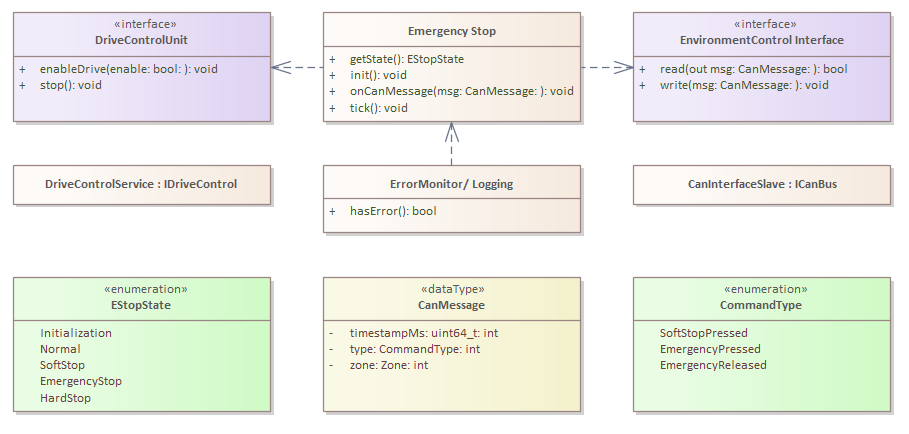
\includegraphics[width=0.95\textwidth]{02_Slave_ClassDiagram}
  \caption{Klassendiagramm Arduino Mega Slave: Sicherheits- und Antriebssubsystem}
  \label{fig:slave_classes}
\end{figure}

Hauptverantwortlichkeiten des Slave-Subsystems:
\begin{description}
  \item[\texttt{EnvironmentControl}]
    Schnittstelle zur Empfangsseite des CAN-Busses; übersetzt eingehende Pakete
    in interne Ereignisse für den Emergency Stop.
  \item[\texttt{EmergencyStop}]
    Zentrale Sicherheitsklasse (Detailed Design in Abschnitt~\ref{sec:detaileddesign}).
    Steuert den Zustandsautomaten und die DriveControlUnit.
  \item[\texttt{DriveControlUnit}]
    Abstrahiert die Motorsteuerung; empfängt ausschließlich Stop-/Freigabe-Befehle
    vom Emergency Stop.
  \item[\texttt{Logger}]
    Querschnittsmodul für Error-Logging; unterstützt Level (\texttt{ERROR},
    \texttt{WARNING}, \texttt{INFO}) mit Zeitstempel.
\end{description}

% =============================================================
%  Kapitel 3 – Verteilungsarchitektur (Deployment)
% =============================================================
\section{Verteilungsarchitektur (Deployment)}
\label{sec:deployment}

Das Deployment-Diagramm (Abbildung~\ref{fig:deployment}) ordnet Softwarekomponenten
den physischen Hardwareeinheiten zu und macht die Kommunikationskanäle sichtbar.

\begin{figure}[H]
  \centering
  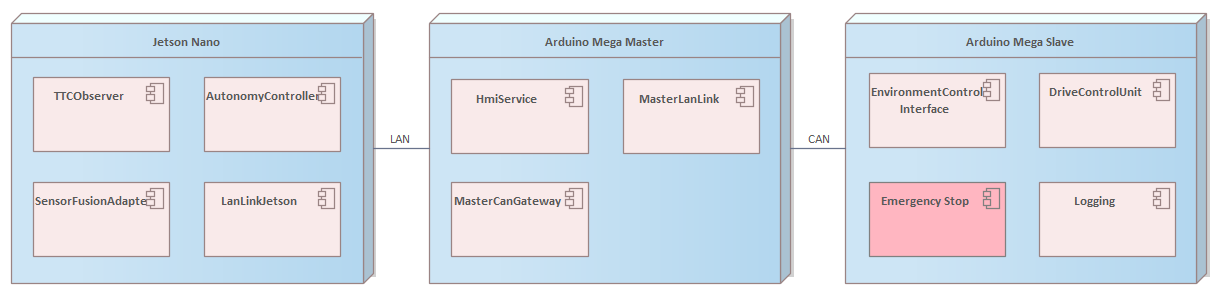
\includegraphics[width=0.95\textwidth]{03_Deployment}
  \caption{Deployment-Diagramm – Hardware/Software-Mapping}
  \label{fig:deployment}
\end{figure}

\subsection{Komponentenverteilung}

\begin{center}
\renewcommand{\arraystretch}{1.3}
\begin{tabular}{>{\bfseries}p{4cm} p{9cm}}
  \toprule
  Hardware-Knoten & Softwarekomponenten \\
  \midrule
  Jetson Nano
    & \texttt{AutonomyController}, \texttt{TTCObserver},
      \texttt{SensorFusionAdapter} \\
  Arduino Mega Master
    & \texttt{MasterLanLink}, \texttt{MasterCanGateway},
      \texttt{HmiService} \\
  Arduino Mega Slave
    & \texttt{EnvironmentControl}, \texttt{EmergencyStop},
      \texttt{DriveControlUnit}, \texttt{Logger} \\
  \bottomrule
\end{tabular}
\end{center}

\subsection{Kommunikationskanäle}

\begin{itemize}
  \item \textbf{LAN} (Ethernet): Jetson Nano $\leftrightarrow$ Arduino Mega Master. \\
    Überträgt Autonomie-Kommandos und Zonen-Updates vom Jetson zum Master.
  \item \textbf{CAN-Bus}: Arduino Mega Master $\leftrightarrow$ Arduino Mega Slave. \\
    Überträgt CAN-Pakete mit Zonenstatus, Emergency-Ereignissen und Steuerbefehlen.
    \assumption{CAN-Datenklasse kapselt Paketstruktur (ID, Payload, Timestamp).}
\end{itemize}

\subsection{Rationale der Verteilung}

Die Platzierung des Emergency Stop direkt auf dem Arduino Mega Slave
neben der \texttt{DriveControlUnit} verfolgt folgende Ziele:

\begin{enumerate}
  \item \textbf{Minimale Latenz:} Kein zusätzlicher Kommunikationsweg zwischen
        Sicherheitslogik und Motorsteuerung.
  \item \textbf{Isolation:} Ausfall des Jetson oder des Masters hat keinen direkten
        Einfluss auf die Fähigkeit, einen Stopp einzuleiten.
  \item \textbf{Determinismus:} Der Slave führt eine einfache Echtzeit-Logik aus;
        kein OS-Overhead wie auf dem Jetson.
\end{enumerate}

\todobox{Latenzzahlen (typische CAN-Zykluszeit, LAN-Latenz) ergänzen,
sobald Messungen vorliegen.}

% =============================================================
%  Kapitel 4 – Dynamisches Verhalten (Global Software Control + Boundary Conditions)
% =============================================================
\section{Dynamisches Verhalten des Systems}
\label{sec:dynamik}

Dieser Abschnitt beschreibt das Laufzeitverhalten anhand von Sequenzdiagrammen.
Er umfasst sowohl den \emph{Global Software Control} (regulärer Betrieb mit
Emergency Stop) als auch die \emph{Boundary Conditions} (Systemstart, Shutdown,
Fehlerbehandlung).

% ------------------------------------------------------------
\subsection{Global Software Control: Auslösung durch Safety-Zone}
\label{sec:seq_safetyzone}

\begin{figure}[H]
  \centering
  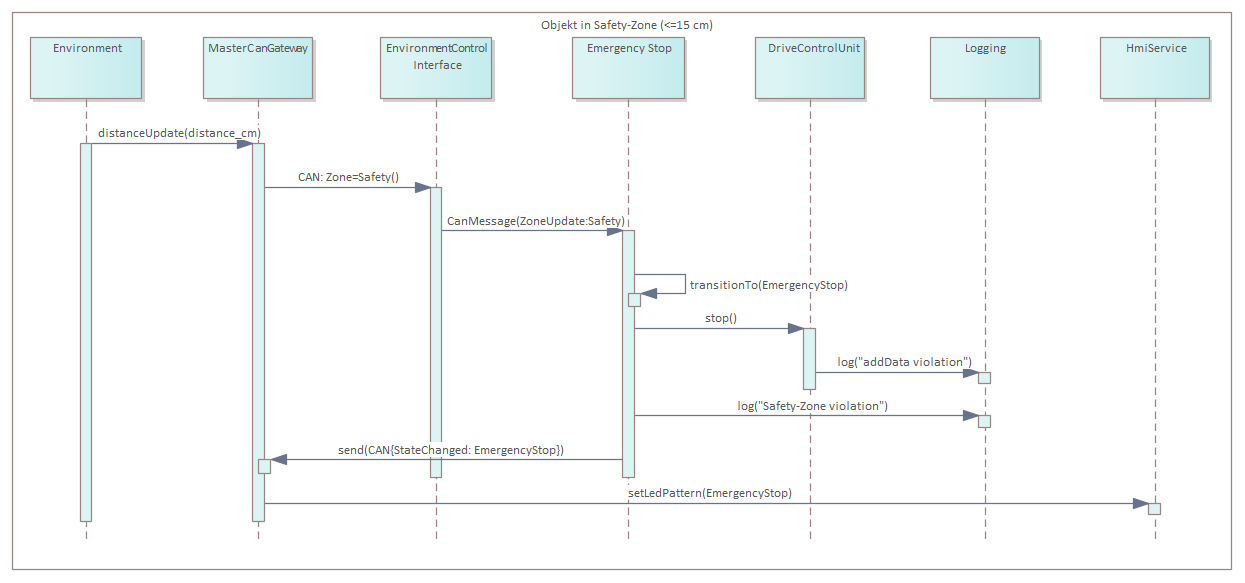
\includegraphics[width=0.95\textwidth]{04_Sequence_SafetyZone}
  \caption{Sequenzdiagramm: Auslösung des Emergency Stop durch Safety-Zone (Rot)}
  \label{fig:seq_safetyzone}
\end{figure}

Wird eine Distanz $\leq 15\,\mathrm{cm}$ erkannt (rote Sicherheitszone), läuft
folgender Ablauf ab (Abbildung~\ref{fig:seq_safetyzone}):

\begin{enumerate}
  \item Der \texttt{SensorFusionAdapter} auf dem Jetson meldet ein Objekt in der
        Safety-Zone.
  \item Der \texttt{TTCObserver} erzeugt ein \texttt{ZoneUpdate(Safety)}-Ereignis.
  \item Über \ac{LAN} $\to$ \texttt{MasterLanLink} $\to$ \texttt{MasterCanGateway}
        wird ein \ac{CAN}-Paket generiert.
  \item Das \ac{CAN}-Paket wird vom \texttt{EnvironmentControl}-Interface auf dem Slave
        empfangen und an \texttt{EmergencyStop} weitergegeben.
  \item Der Emergency Stop wechselt in den Zustand \texttt{EmergencyStop},
        sendet einen \textbf{Stop-Befehl} an die \texttt{DriveControlUnit}
        und löst einen \texttt{Logger.log(ERROR, "Safety zone triggered")}-Aufruf aus.
  \item Die Status-\ac{LED} wechselt auf Rot.
\end{enumerate}

\textbf{Wichtig:} Das Fahrzeug bleibt blockiert, bis eine manuelle Freigabe
die Guard-Bedingung erfüllt (vgl.\ Abschnitt~\ref{sec:seq_release}).

% ------------------------------------------------------------
\subsection{Boundary Condition: Systemstart (Startup)}
\label{sec:seq_startup}

\begin{figure}[H]
  \centering
  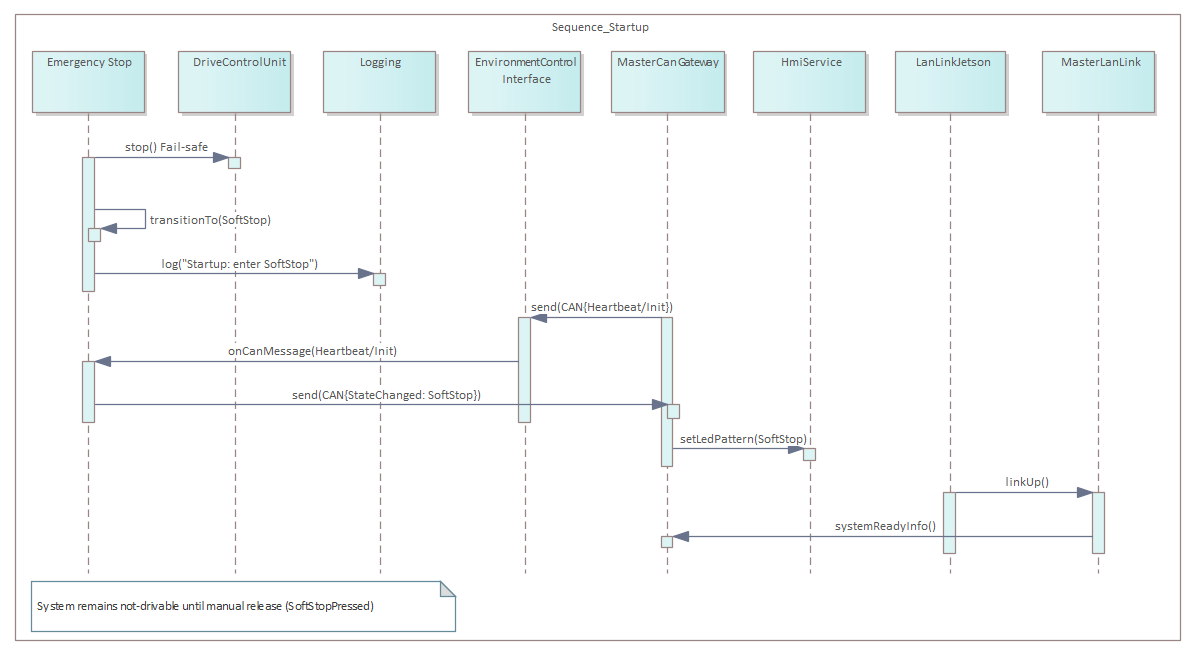
\includegraphics[width=0.95\textwidth]{05_Sequence_Startup}
  \caption{Sequenzdiagramm: Startup-Verhalten}
  \label{fig:seq_startup}
\end{figure}

Beim Systemstart (Abbildung~\ref{fig:seq_startup}) werden alle Komponenten initialisiert.
Der Emergency Stop beginnt automatisch im Zustand \texttt{SoftStop}
(\emph{Safe-Default}): Das Fahrzeug ist erst nach einer expliziten
manuellen Freigabe fahrbereit.

\textbf{Ablauf:}
\begin{enumerate}
  \item Alle Hardware-Einheiten starten ihre Initialisierungsroutine.
  \item \texttt{EmergencyStop} wechselt von \texttt{Initialization}
        nach \texttt{SoftStop}.
  \item \texttt{Logger} registriert \texttt{INFO: System startup complete}.
  \item Fahrzeug wartet auf Freigabe-Signal (Taster/Button).
\end{enumerate}

% ------------------------------------------------------------
\subsection{Boundary Condition: Freigabe nach Emergency Stop (Release)}
\label{sec:seq_release}

\begin{figure}[H]
  \centering
  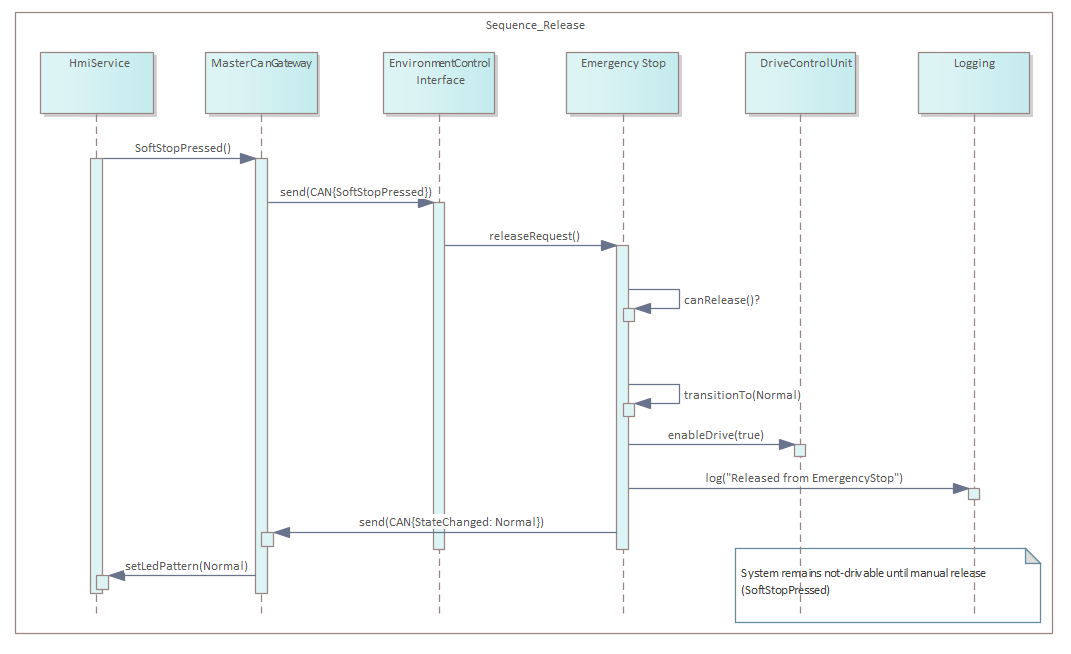
\includegraphics[width=0.95\textwidth]{05_Sequence_Release}
  \caption{Sequenzdiagramm: Manuelle Freigabe nach Emergency Stop}
  \label{fig:seq_release}
\end{figure}

Nach einem Emergency Stop ist eine manuelle Freigabe erforderlich (Abbildung~\ref{fig:seq_release}).
Die Guard-Bedingung muss vollständig erfüllt sein:

\begin{itemize}
  \item Safety-Zone ist \textbf{nicht} mehr aktiv (kein Objekt in Rot).
  \item Kein Fehler ist aktiv (\texttt{errorFlag == false}).
\end{itemize}

Erst dann erfolgt:
\begin{enumerate}
  \item Zustandswechsel \texttt{EmergencyStop} $\to$ \texttt{Normal}.
  \item Aktivierung der \texttt{DriveControlUnit} (Freigabe der Motorsteuerung).
  \item \texttt{Logger.log(INFO, "System released, resuming normal operation")}.
\end{enumerate}

% ------------------------------------------------------------
\subsection{Boundary Condition: Freigabe abgelehnt (Release Rejected)}
\label{sec:seq_releaserejected}

\begin{figure}[H]
  \centering
  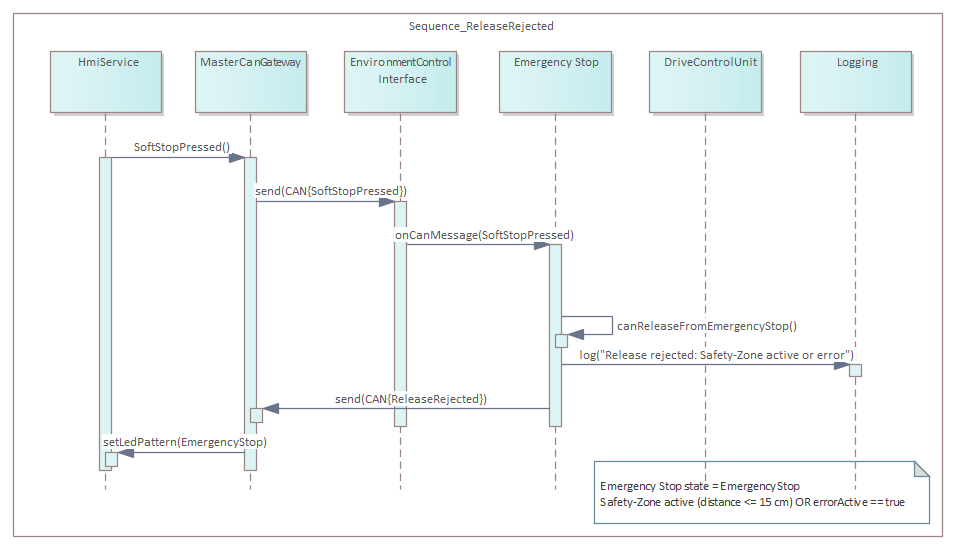
\includegraphics[width=0.95\textwidth]{05_Sequence_ReleaseRejected}
  \caption{Sequenzdiagramm: Freigabe abgelehnt (Guard nicht erfüllt)}
  \label{fig:seq_releaserejected}
\end{figure}

Ist die Safety-Zone noch aktiv oder liegt ein Fehler vor,
wird der Freigabe-Request \textbf{abgelehnt} (Abbildung~\ref{fig:seq_releaserejected}).
Der Zustand bleibt unverändert (\texttt{EmergencyStop}).
\texttt{Logger} protokolliert \texttt{WARNING: Release rejected – condition not met}.

% ------------------------------------------------------------
\subsection{Boundary Condition: Fehlerbehandlung (Error)}
\label{sec:seq_error}

\begin{figure}[H]
  \centering
  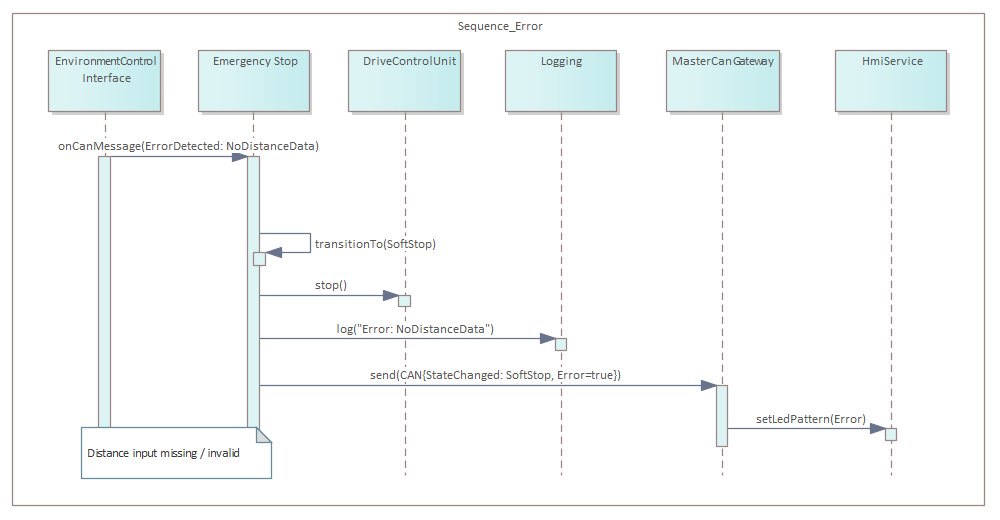
\includegraphics[width=0.95\textwidth]{05_Sequence_Error}
  \caption{Sequenzdiagramm: Fehlerbehandlung (fehlende Sensordaten)}
  \label{fig:seq_error}
\end{figure}

Fehlen gültige Sensordaten (z.\,B.\ LiDAR-Ausfall, \ac{CAN}-Timeout),
greift das \textbf{Fail-Safe-Prinzip} (Abbildung~\ref{fig:seq_error}):

\begin{enumerate}
  \item \texttt{EnvironmentControl} detektiert fehlende/ungültige \ac{CAN}-Daten.
  \item \texttt{EmergencyStop} erhält \texttt{ErrorDetected}-Ereignis.
  \item Zustandswechsel nach \texttt{SoftStop} (falls noch nicht gestoppt).
  \item \texttt{Logger.log(ERROR, "Sensor data missing – soft stop engaged")}.
\end{enumerate}

\textbf{Regel:} Keine gültigen Daten $\Rightarrow$ Stopp + Logging (keine Ausnahmen).

% ------------------------------------------------------------
\subsection{Boundary Condition: Shutdown}
\label{sec:seq_shutdown}

\begin{figure}[H]
  \centering
  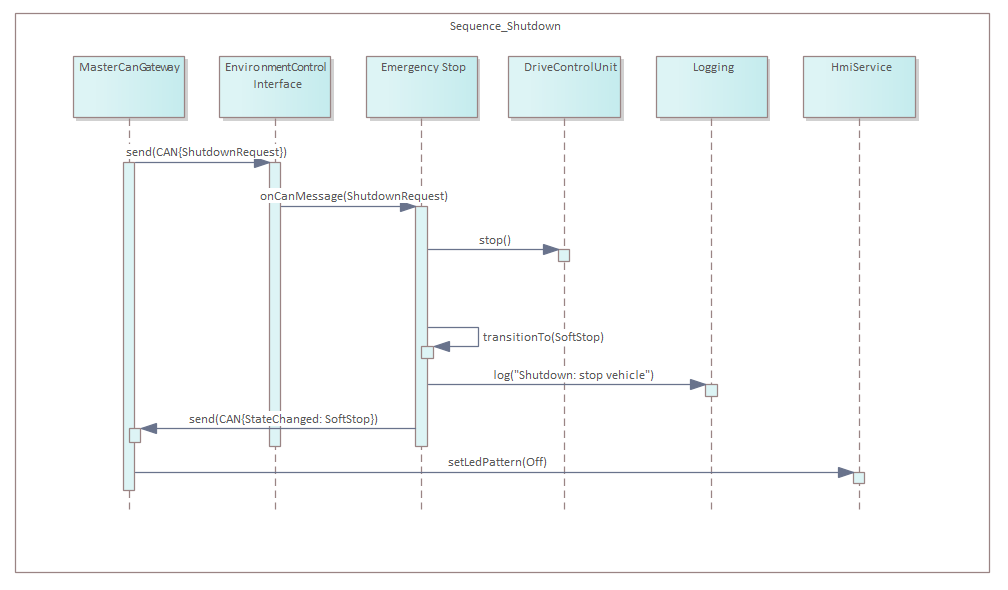
\includegraphics[width=0.95\textwidth]{05_Sequence_Shutdown}
  \caption{Sequenzdiagramm: Kontrollierter Shutdown}
  \label{fig:seq_shutdown}
\end{figure}

Bei einem \texttt{ShutdownRequest} (Abbildung~\ref{fig:seq_shutdown}):
\begin{enumerate}
  \item \texttt{EmergencyStop} empfängt das Shutdown-Ereignis.
  \item Zustandswechsel nach \texttt{SoftStop}.
  \item Stop-Befehl an \texttt{DriveControlUnit}.
  \item \texttt{Logger.log(INFO, "Shutdown initiated")}.
  \item Alle Subsysteme fahren geordnet herunter.
\end{enumerate}

% =============================================================
%  Kapitel 5 – Detailed Design: Emergency Stop
% =============================================================
\section{Detailed Design: Emergency Stop}
\label{sec:detaileddesign}

Dieser Abschnitt fokussiert ausschließlich auf das
\texttt{EmergencyStop}-Modul und beschreibt sein Klassendesign,
den internen Ablauf sowie den vollständigen Zustandsautomaten.

% ------------------------------------------------------------
\subsection{Klassendesign}
\label{sec:estop_klassen}

\begin{figure}[H]
  \centering
  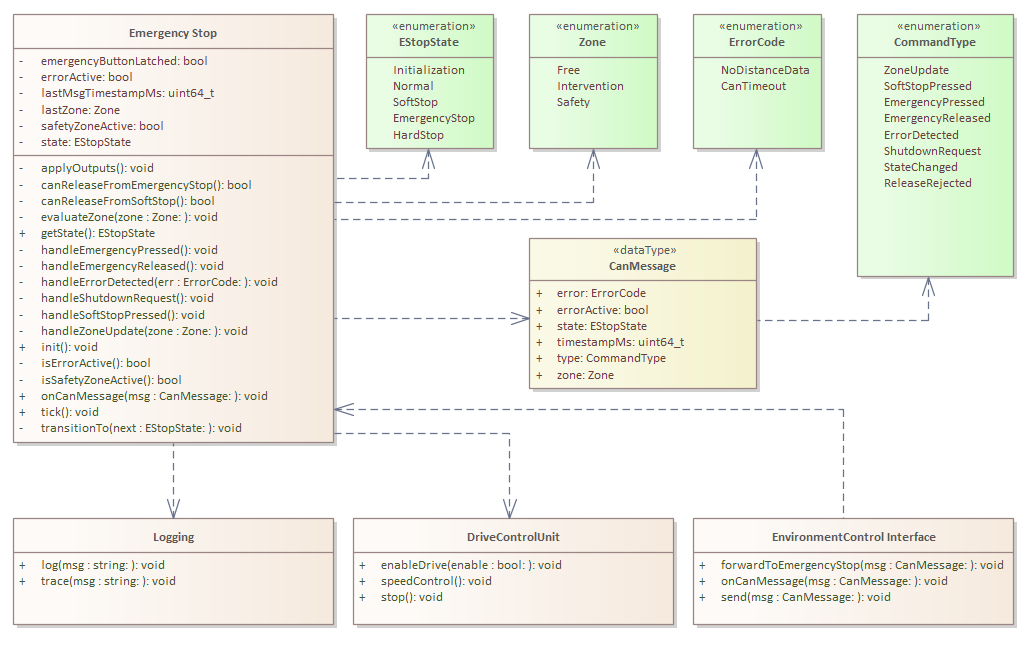
\includegraphics[width=0.95\textwidth]{06_EStop_Class_Detailed}
  \caption{Detailliertes Klassendiagramm – EmergencyStop inkl.\ private Methoden}
  \label{fig:estop_class}
\end{figure}

Die Klasse \texttt{EmergencyStop} kapselt den vollständigen Sicherheitszustand.

\subsubsection{Attribute}

\begin{center}
\renewcommand{\arraystretch}{1.3}
\begin{tabular}{>{\ttfamily}p{4.5cm} >{\ttfamily}p{3cm} p{6cm}}
  \toprule
  \normalfont\textbf{Name} & \normalfont\textbf{Typ} & \normalfont\textbf{Beschreibung} \\
  \midrule
  currentState   & EStopState  & Aktueller Zustand des Automaten \\
  errorFlag      & bool        & Aktiver Fehler vorhanden \\
  safetyZoneActive & bool      & Safety-Zone (Rot) gerade aktiv \\
  driveRef       & DriveControlUnit* & Referenz auf Motorsteuerung \\
  loggerRef      & Logger*     & Referenz auf Logging-Modul \\
  \bottomrule
\end{tabular}
\end{center}

\subsubsection{Öffentliche Operationen (Public Interface)}

\begin{center}
\renewcommand{\arraystretch}{1.3}
\begin{tabular}{>{\ttfamily}p{6.5cm} p{7cm}}
  \toprule
  \normalfont\textbf{Signatur} & \normalfont\textbf{Beschreibung} \\
  \midrule
  onZoneUpdate(zone: Zone) : void
    & Eingehende Zonenänderung verarbeiten (Safety / Normal). \\
  onEmergencyButton() : void
    & Pilzknopf-Event verarbeiten. \\
  onFrontTrigger() : void
    & Fronttaster-Event verarbeiten. \\
  onReleaseRequest() : void
    & Manuelle Freigabe anfordern; Guard wird geprüft. \\
  onErrorDetected() : void
    & Fehler-Ereignis (z.\,B.\ fehlende Sensordaten) verarbeiten. \\
  onShutdownRequest() : void
    & Kontrollierter Shutdown einleiten. \\
  \bottomrule
\end{tabular}
\end{center}

\subsubsection{Private Methoden}

Alle internen Handler sind als \textbf{private Methoden} implementiert,
um die Kapselung der Zustandslogik zu gewährleisten.

\begin{center}
\renewcommand{\arraystretch}{1.3}
\begin{tabular}{>{\ttfamily}p{6.5cm} p{7cm}}
  \toprule
  \normalfont\textbf{Signatur} & \normalfont\textbf{Beschreibung} \\
  \midrule
  triggerEmergencyStop() : void
    & Setzt Zustand auf \texttt{EmergencyStop}; ruft \texttt{stopDrive()} auf. \\
  triggerSoftStop() : void
    & Setzt Zustand auf \texttt{SoftStop}; ruft \texttt{stopDrive()} auf. \\
  stopDrive() : void
    & Sendet Stop-Befehl an \texttt{DriveControlUnit}. \\
  enableDrive() : void
    & Sendet Freigabe-Befehl an \texttt{DriveControlUnit}. \\
  checkReleaseGuard() : bool
    & Prüft: \texttt{!safetyZoneActive \&\& !errorFlag}. \\
  logEvent(level: LogLevel, msg: string) : void
    & Delegiert an \texttt{Logger}; fügt Zeitstempel hinzu. \\
  transitionTo(state: EStopState) : void
    & Führt Zustandsübergang durch und protokolliert ihn. \\
  \bottomrule
\end{tabular}
\end{center}

\subsubsection{Enum: EStopState}

\begin{center}
\renewcommand{\arraystretch}{1.2}
\begin{tabular}{>{\ttfamily}p{4cm} p{9cm}}
  \toprule
  \normalfont\textbf{Wert} & \normalfont\textbf{Bedeutung} \\
  \midrule
  Initialization & Startphase; alle Aktuatoren gesperrt. \\
  SoftStop       & Sicherer Stopp; automatisch wiederherstellbar nach Freigabe. \\
  Normal         & Normalbetrieb; \texttt{DriveControlUnit} freigegeben. \\
  EmergencyStop  & Notfall-Stopp; blockiert bis manuelle Freigabe + Guard-Check. \\
  HardStop       & Höchste Priorität; hardware-seitiger Stopp (kein SW-Override). \\
  \bottomrule
\end{tabular}
\end{center}

\todobox{Vollständige Liste aller privaten Methoden mit Vor-/Nachbedingungen
(Design by Contract) noch auszuarbeiten.}

% ------------------------------------------------------------
\subsection{Interner Ablauf (Sequenzdiagramm)}
\label{sec:estop_seq}

\begin{figure}[H]
  \centering
  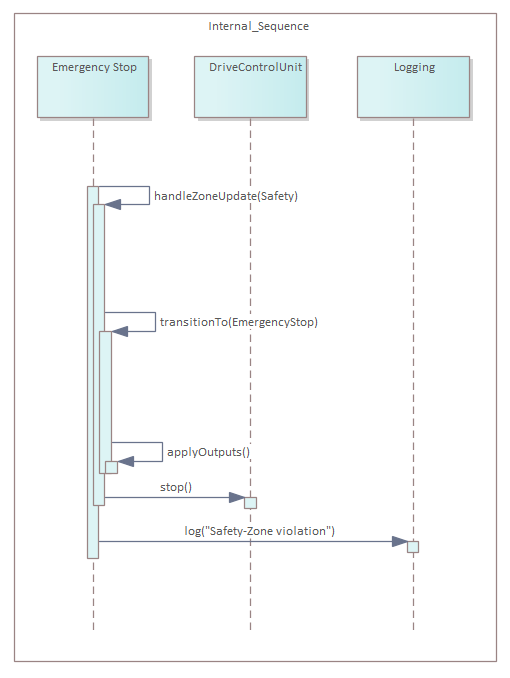
\includegraphics[width=0.95\textwidth]{06_EStop_Internal_Sequence}
  \caption{Internes Sequenzdiagramm – Ablauf innerhalb von EmergencyStop}
  \label{fig:estop_seq}
\end{figure}

Das interne Sequenzdiagramm (Abbildung~\ref{fig:estop_seq}) zeigt,
wie ein eingehender Event durch die privaten Methoden verarbeitet wird.
Die Verarbeitung folgt immer dem gleichen Schema:

\begin{enumerate}
  \item \textbf{Event-Empfang} über eine öffentliche Methode
        (z.\,B.\ \texttt{onZoneUpdate()}).
  \item \textbf{Guard-Prüfung} (falls erforderlich) durch \texttt{checkReleaseGuard()}.
  \item \textbf{Zustandsübergang} über \texttt{transitionTo()} mit automatischem Logging.
  \item \textbf{Aktorsteuerung}: Aufruf von \texttt{stopDrive()} oder \texttt{enableDrive()}.
  \item \textbf{Logging} über \texttt{logEvent()} mit Level und Zeitstempel.
\end{enumerate}

Diese Trennung hält die Event-Handler frei von direkten Hardware-Zugriffen
und ermöglicht einfaches Unit-Testing.

% ------------------------------------------------------------
\subsection{Zustandsautomat (State Machine)}
\label{sec:estop_statemachine}

\begin{figure}[H]
  \centering
  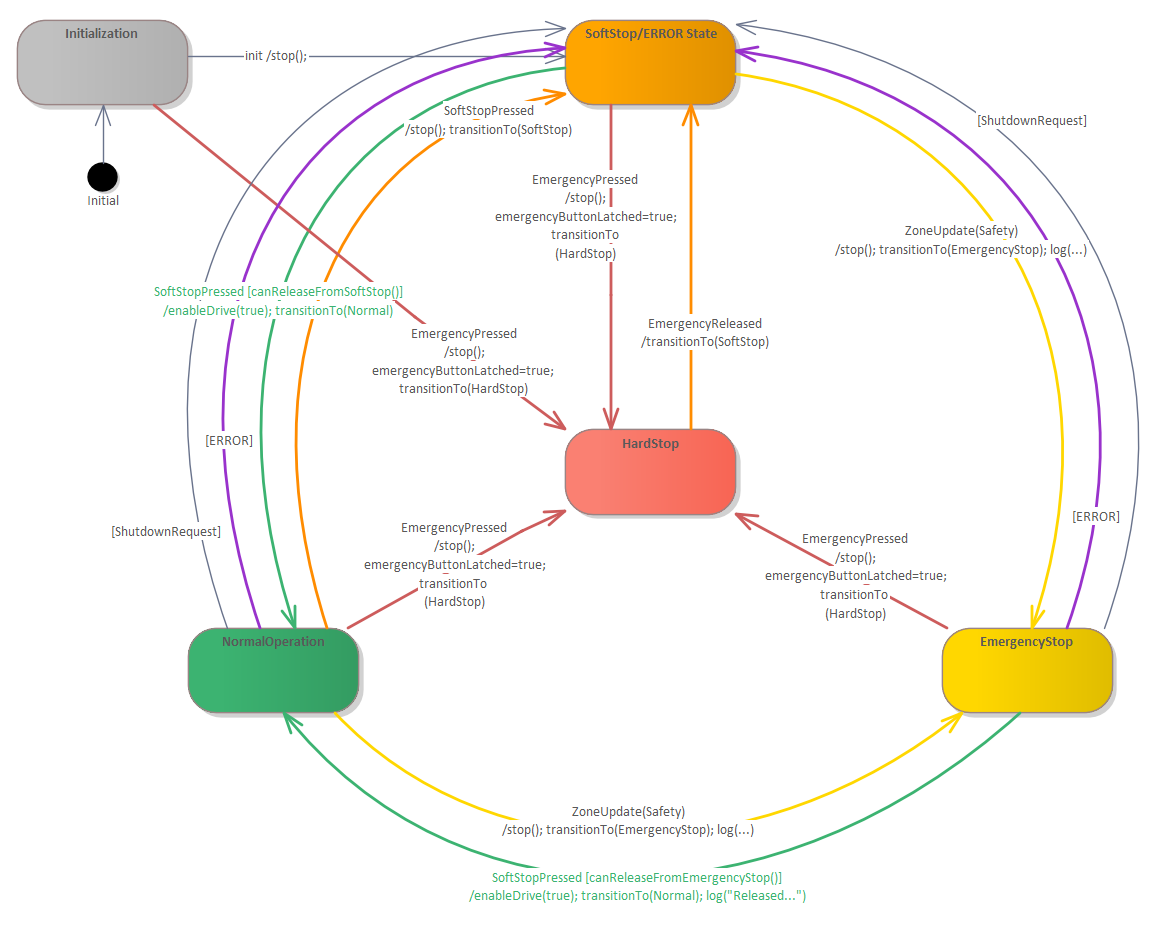
\includegraphics[width=0.95\textwidth]{06_EStop_StateMachine}
  \caption{Zustandsautomat – vollständiges Verhalten von EmergencyStop}
  \label{fig:estop_statemachine}
\end{figure}

Der Zustandsautomat (Abbildung~\ref{fig:estop_statemachine}) definiert das
vollständige Verhalten von \texttt{EmergencyStop}.

\subsubsection{Zustandsübergänge}

\begin{center}
\renewcommand{\arraystretch}{1.3}
\begin{tabular}{>{\ttfamily}p{3.5cm} p{4cm} >{\ttfamily}p{3.5cm}}
  \toprule
  \normalfont\textbf{Von} & \normalfont\textbf{Trigger / Guard} & \normalfont\textbf{Nach} \\
  \midrule
  Initialization    & SystemReady                          & SoftStop \\
  SoftStop          & ReleaseRequest [Guard OK]            & Normal \\
  Normal            & ZoneUpdate(Safety)                   & EmergencyStop \\
  Normal            & EmergencyButton / FrontTrigger       & EmergencyStop \\
  Normal            & ErrorDetected                        & SoftStop \\
  Normal            & ShutdownRequest                      & SoftStop \\
  EmergencyStop     & ReleaseRequest [Guard OK]            & Normal \\
  EmergencyStop     & ReleaseRequest [Guard FAIL]          & EmergencyStop \\
  EmergencyStop     & ErrorDetected                        & SoftStop \\
  SoftStop          & ErrorDetected                        & SoftStop \\
  * (alle)          & HardStopSignal                       & HardStop \\
  \bottomrule
\end{tabular}
\end{center}

\subsubsection{Besondere Eigenschaften}

\begin{itemize}
  \item \textbf{HardStop} hat die höchste Priorität; er kann aus jedem Zustand
        erreicht werden und ist nicht softwareseitig aufhebbar.
  \item \textbf{EmergencyStop} erfordert zwingend eine manuelle Freigabe plus
        erfolgreiche Guard-Prüfung.
  \item \textbf{ErrorDetected} führt immer zu \texttt{SoftStop}
        (Fail-Safe-Prinzip).
  \item \textbf{ShutdownRequest} führt immer zu \texttt{SoftStop}.
\end{itemize}

\todobox{Activity-Diagramme für die wichtigsten privaten Methoden
(\texttt{checkReleaseGuard}, \texttt{triggerEmergencyStop}) ausarbeiten
oder begründen, warum die State-Machine hinreichend ist.}

% =============================================================
%  Kapitel 6 – Architektonische Entscheidungen
% =============================================================
\section{Architektonische Entscheidungen}
\label{sec:entscheidungen}

% ------------------------------------------------------------
\subsection{Sprachauswahl: C vs.\ C++}
\label{sec:sprachauswahl}

\begin{center}
\renewcommand{\arraystretch}{1.4}
\begin{tabular}{>{\bfseries}p{3.5cm} p{5.5cm} p{5.5cm}}
  \toprule
  & \textbf{C} & \textbf{C++} \\
  \midrule
  Vorteile
    & Volle Kontrolle, minimaler Overhead, weit verbreitet auf Embedded \\
    & OOP (Klassen, Vererbung), STL, bessere Kapselung, Lesbarkeit \\
  Nachteile
    & Keine Objektorientierung, schlechte Kapselung, fehleranfälliger Code \\
    & Leicht erhöhter Code-Footprint, RTTI/Exceptions ggf.\ deaktivieren \\
  Eignung Arduino Mega
    & Ja
    & Ja (Arduino-Framework basiert auf C++) \\
  Eignung Jetson Nano
    & Ja
    & Ja \\
  \bottomrule
\end{tabular}
\end{center}

\textbf{Entscheidung: C++}

Das gesamte Systemdesign ist objektorientiert modelliert
(Klassen, Interfaces, Enums); C++ erlaubt eine direkte 1:1-Abbildung
dieses UML-Designs in Code ohne strukturelle Kompromisse.
Da das Arduino-Framework selbst auf C++ basiert
(z.\,B.\ \texttt{HardwareSerial}, \texttt{Stream} als C++-Klassen)
und der Jetson Nano Linux mit vollem C++-Support ausführt,
ist C++ auf allen drei Zielplattformen nativ verfügbar.
Zur Minimierung des Speicher- und Laufzeit-Overheads werden
Exceptions und RTTI im Compiler deaktiviert (\texttt{-fno-exceptions
-fno-rtti}), was auf Arduino-Targets Standard ist.
Insgesamt bietet C++ gegenüber reinem C eine deutlich bessere
Kapselung (z.\,B.\ private Methoden in \texttt{EmergencyStop})
bei vernachlässigbarem Mehraufwand.

\textbf{Verworfene Alternativen:}
Reines C würde alle Klassen als Structs mit Funktionszeigern
erfordern – erheblich mehr Boilerplate ohne architektonischen Mehrwert.
Rust wäre sicherheitstechnisch attraktiv, ist aber auf den
verwendeten Arduino-Targets nicht offiziell unterstützt.

% ------------------------------------------------------------
\subsection{Verteilte Architektur}
\label{sec:entsch_verteilung}

\textbf{Entscheidung:} Drei getrennte Recheneinheiten (Jetson, Master, Slave)
statt Mono-Architektur.

\textbf{Rationale:}
\begin{itemize}
  \item \emph{Separation of Concerns:} Wahrnehmung (Jetson) und Sicherheit (Slave)
        sind physisch und softwareseitig getrennt.
  \item \emph{Determinismus:} Der Slave führt eine einfache Regellogik ohne
        OS-Overhead aus.
  \item \emph{Fault Isolation:} Ein Absturz des Jetson deaktiviert den Emergency Stop
        nicht (Fail-Safe: Slave stoppt selbstständig bei ausbleibenden Daten).
\end{itemize}

\textbf{Alternative:} Alles auf dem Jetson Nano (Mono-Architektur).
Wurde verworfen, da dies einen Single Point of Failure schafft und
die Reaktionszeit durch OS-Scheduling unvorhersehbar wird.

% ------------------------------------------------------------
\subsection{Fail-Safe-Prinzip}
\label{sec:entsch_failsafe}

\textbf{Entscheidung:} Im Zweifel immer stoppen.

Konkrete Umsetzungen:
\begin{itemize}
  \item Startup beginnt in \texttt{SoftStop} (kein automatisches Losfahren).
  \item Fehlende Sensordaten $\Rightarrow$ \texttt{SoftStop} + Logging.
  \item \texttt{HardStop} ist von keiner Zustand aus aufhebbar.
\end{itemize}

% ------------------------------------------------------------
\subsection{Klare Verantwortlichkeiten}
\label{sec:entsch_verantwortlichkeiten}

\begin{center}
\renewcommand{\arraystretch}{1.3}
\begin{tabular}{>{\bfseries}p{4cm} p{9.5cm}}
  \toprule
  Komponente & Alleinige Verantwortlichkeit \\
  \midrule
  TTCObserver     & Normal Operation (Gelb/Grün); kein Zugriff auf Emergency Stop. \\
  EmergencyStop   & Sicherheits-Zustände (Rot, Knopf, Taster); kein Zugriff auf TTC. \\
  Logger          & Persistentes Logging; keine Entscheidungslogik. \\
  DriveControlUnit & Motorsteuerung; reagiert nur auf explizite Stop-/Go-Befehle. \\
  \bottomrule
\end{tabular}
\end{center}

% ------------------------------------------------------------
\subsection{CAN als Kommunikationsprotokoll}
\label{sec:entsch_can}

\textbf{Rationale:} CAN ist für Automotive-Systeme optimiert, bietet priorisierungsbasierte
Arbitrierung und eine hardware-gesicherte Fehlerkennung (CRC, ACK). Dies passt besser
zu den Echtzeit-Anforderungen einer Sicherheitsfunktion als eine LAN-basierte Lösung.

\assumption{CAN-Zykluszeit $< 5\,\mathrm{ms}$; konkrete Werte aus Systemtest nachzutragen.}

% =============================================================
%  Kapitel 7 – Traceability: Anforderung → Artefakt
% =============================================================
\section{Traceability: Anforderung \texorpdfstring{$\to$}{->} Artefakt}
\label{sec:traceability}

Die folgende Tabelle ordnet jede Pflichtanforderung der Aufgabenstellung
einem konkreten Artefakt in diesem Dokument zu.

\begin{center}
\renewcommand{\arraystretch}{1.4}
\begin{longtable}{p{6.5cm} p{4.5cm} p{2.5cm}}
  \toprule
  \textbf{Anforderung (Aufgabenstellung)} &
  \textbf{Artefakt / Diagramm} &
  \textbf{Abschnitt} \\
  \midrule
  \endhead
  % --- Architektur ---
  Architektur-Übersicht (Context Diagram)
    & Abb.~\ref{fig:context} \newline 01\_Context.png
    & \S\,\ref{sec:systemkontext} \\
  Subsystem-Zerlegung + Verantwortlichkeiten
    & Abb.~\ref{fig:component_overview} \newline 02\_Component\_Overview.png
    & \S\,\ref{sec:component_overview} \\
  Class Diagrams (Jetson)
    & Abb.~\ref{fig:jetson_classes} \newline 02\_Jetson\_ClassDiagram.png
    & \S\,\ref{sec:klassendiagramme} \\
  Class Diagrams (Master)
    & Abb.~\ref{fig:master_classes} \newline 02\_Master\_ClassDiagram.png
    & \S\,\ref{sec:klassendiagramme} \\
  Class Diagrams (Slave)
    & Abb.~\ref{fig:slave_classes} \newline 02\_Slave\_ClassDiagram.png
    & \S\,\ref{sec:klassendiagramme} \\
  % --- Deployment ---
  Hardware/Software-Mapping (Deployment)
    & Abb.~\ref{fig:deployment} \newline 03\_Deployment.png
    & \S\,\ref{sec:deployment} \\
  % --- Global Software Control ---
  Global Software Control (Sequenz Safety-Zone)
    & Abb.~\ref{fig:seq_safetyzone} \newline 04\_Sequence\_SafetyZone.png
    & \S\,\ref{sec:seq_safetyzone} \\
  % --- Boundary Conditions ---
  Boundary Condition: Startup
    & Abb.~\ref{fig:seq_startup} \newline 05\_Sequence\_Startup.png
    & \S\,\ref{sec:seq_startup} \\
  Boundary Condition: Shutdown
    & Abb.~\ref{fig:seq_shutdown} \newline 05\_Sequence\_Shutdown.png
    & \S\,\ref{sec:seq_shutdown} \\
  Boundary Condition: Error
    & Abb.~\ref{fig:seq_error} \newline 05\_Sequence\_Error.png
    & \S\,\ref{sec:seq_error} \\
  Boundary Condition: Release
    & Abb.~\ref{fig:seq_release} \newline 05\_Sequence\_Release.png
    & \S\,\ref{sec:seq_release} \\
  Boundary Condition: Release Rejected
    & Abb.~\ref{fig:seq_releaserejected} \newline 05\_Sequence\_ReleaseRejected.png
    & \S\,\ref{sec:seq_releaserejected} \\
  % --- Detailed Design ---
  Detailed Design ES: Klasse + private Methoden
    & Abb.~\ref{fig:estop_class} \newline 06\_EStop\_Class\_Detailed.png + Tabellen
    & \S\,\ref{sec:estop_klassen} \\
  Detailed Design ES: Internes Sequenzdiagramm
    & Abb.~\ref{fig:estop_seq} \newline 06\_EStop\_Internal\_Sequence.png
    & \S\,\ref{sec:estop_seq} \\
  Detailed Design ES: State Machine
    & Abb.~\ref{fig:estop_statemachine} \newline 06\_EStop\_StateMachine.png
    & \S\,\ref{sec:estop_statemachine} \\
  % --- Entscheidungen ---
  Sprachauswahl (C vs.\ C++) + Rationale
    & Text + Tabelle
    & \S\,\ref{sec:sprachauswahl} \\
  Architektur-Alternativen + Rationale
    & Text
    & \S\,\ref{sec:entsch_verteilung} \\
  % --- Offene Punkte ---
  Activity-Diagramme pro private Methode
    & \todo{Ausstehend}
    & \S\,\ref{sec:naechste_schritte} \\
  \bottomrule
\end{longtable}
\end{center}

% =============================================================
%  Kapitel 8 – Nächste Schritte / Offene Punkte
% =============================================================
\section{Nächste Schritte und offene Punkte}
\label{sec:naechste_schritte}

Die folgende Liste fasst die wichtigsten offenen Punkte zusammen,
priorisiert nach Relevanz für die Bewertung.

\subsection{Priorisierte To-do-Liste}

\begin{enumerate}
  \item \textbf{[P1 – Detailed Design]}
    \textbf{Activity-Diagramme für private Methoden ausarbeiten.} \\
    Mindestens für \texttt{checkReleaseGuard()} und
    \texttt{triggerEmergencyStop()} ein Activity-Diagramm erstellen
    \emph{oder} schriftlich begründen, warum der Zustandsautomat
    (Abschnitt~\ref{sec:estop_statemachine}) als alleinige
    dynamische Modellierung ausreicht.
    \todo{Activity-Diagramme erstellen oder Begründung formulieren.}

  \item \textbf{[P1 – Detailed Design]}
    \textbf{Vollständige Methodenliste mit Vor-/Nachbedingungen.} \\
    Alle privaten Methoden der Klasse \texttt{EmergencyStop} mit
    Preconditions, Postconditions und ggf.\ Invarianten spezifizieren
    (Design by Contract).
    \todo{Tabelle mit Pre-/Postconditions für alle privaten Methoden vervollständigen.}

  \item \textbf{[P2 – Architektur]}
    \textbf{Kurze schriftliche Begründung der Sprachauswahl (C++) finalisieren.} \\
    Der Abschnitt~\ref{sec:sprachauswahl} enthält bereits die wesentlichen
    Argumente. Mit dem Team abstimmen und auf 3--5 Sätze verdichten.
    \todo{Sprachauswahl-Begründung mit Team abstimmen und finalisieren.}

  \item \textbf{[P2 – Architektur]}
    \textbf{CAN-Datenklasse ausdetaillieren.} \\
    Die Klasse für CAN-Pakete (Struktur: ID, Payload, Timestamp) in einem
    eigenen Klassendiagramm modellieren und in Abschnitt~\ref{sec:klassendiagramme}
    einbinden.
    \todo{CAN-Datenklasse modellieren und Diagramm einbinden.}

  \item \textbf{[P3 – Qualität]}
    \textbf{Latenzzahlen ergänzen.} \\
    Typische CAN-Zykluszeit und LAN-Latenz aus Systemtests eintragen
    (Abschnitt~\ref{sec:deployment}).
    \todo{Messwerte aus Systemtest nachtragen.}

  \item \textbf{[P3 – Optional]}
    \textbf{Logger-Interface vollständig spezifizieren.} \\
    Vollständige Methodenliste für \texttt{Logger} (inkl.\ Log-Level-Enum,
    Puffer-Strategie, Ausgabe-Kanal).
    \todo{Logger-Interface ausarbeiten (optional, aber gern gesehen laut Aufgabenstellung).}

  \item \textbf{[P3 – Optional]}
    \textbf{Interfaces (\texttt{EnvironmentControl}) vollständig ausarbeiten.} \\
    Nicht nur eine einzelne Funktion, sondern alle Methoden und Signale
    des Interfaces spezifizieren.
    \todo{EnvironmentControl-Interface vollständig modellieren.}
\end{enumerate}

\subsection{Bekannte Annahmen (zur Überprüfung)}

Die folgenden Annahmen wurden getroffen und müssen mit dem Team
bzw.\ der Aufgabenstellung validiert werden:

\begin{itemize}
  \item \assumption{Emergency Stop läuft auf dem Arduino Mega Slave
        (nahe DriveControlUnit). Erste Vermutung laut Mitschrieb; zu bestätigen.}
  \item \assumption{CAN-Zykluszeit $< 5\,\text{ms}$; zu messen.}
  \item \assumption{Distanzschwelle für Rot-Zone: $\leq 15\,\mathrm{cm}$.}
  \item \assumption{CAN-Datenklasse kapselt ID, Payload und Timestamp.}
  \item \assumption{Logger schreibt auf seriellen Ausgang des Slave-Arduinos;
        kein persistenter Speicher.}
\end{itemize}


\end{document}
